% !TEX root = slides_ISSTA.tex
\subsection{Developer Survey}

\begin{frame}
\frametitle{Part 1: Context}

\begin{block}{RQ1}
In what contexts do professional developers use regular expressions?
\end{block}
\end{frame}

\begin{frame}
\frametitle{Survey context}

\begin{itemize}
	\item 18 professional developers 
	\item 9 years average development experience
	\item Small mobile payment management company
	\item 30 questions in a Google form
\end{itemize}
\end{frame}

\begin{frame}
\frametitle{How often and where do developers use regexes?}

\begin{itemize}
	\item 50\%  -- at least once per week
%	\item 100\% -- at least once per month
\vspace{12pt}
	\item<2-> {\bf Most often}: command line and text editor tools
	\item<2-> {\bf Often}: general purpose and scripting  languages
%	\item 2 developers write more than 50 regexes annually in general programming languages (e.g., Java) 
	\item<2-> {\bf Rare}: Database queries
\end{itemize}
\end{frame}


%\begin{frame}
%\frametitle{Common regex activities}
%
%\begin{block}{How often do you use regexes for... }
%
%\begin{center}
%\begin{tabular}{l|c}
%\toprule
%\textbf{Activity} & \textbf{Frequency} \\  \hline 
%Locating content within a file or files & 4.4\\ \hline 
%Capturing parts of strings & 4.3 \\ \hline 
%Parsing user input & 4.0\\  \hline
%Counting lines that match a pattern & 3.2 \\ \hline
%Checking for a single character & 1.7\\ \hline
%\bottomrule
%\end{tabular}
%\end{center}
%\end{block}
%\textcolor{red}{Key: 6 = very frequently, 5 = frequently, 4 = occasionally, \\3 = rarely, 2 = very rarely, 1 = never}
%
%\end{frame}


%{
%\setbeamertemplate{background canvas}{\tikz[remember picture]\node[opacity=0.5] at (current page.center) {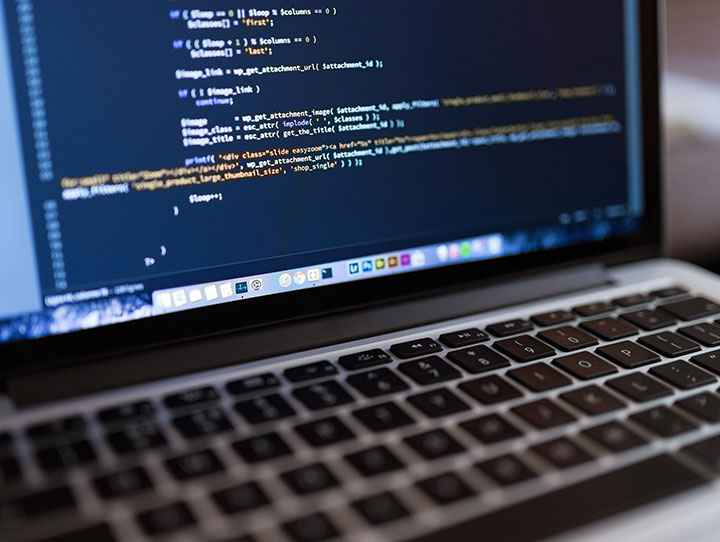
\includegraphics[height=1.055\textheight,keepaspectratio]{nontex/illustrations/pexels-photoSmall.jpg}};}
%\begin{frame}
%\frametitle{How Do Developers Say They Use Regexes?}
%\begin{block}{\begin{Large}Developer Input On Regex Usage Is Missing\end{Large}}
%\begin{itemize}
%\item \begin{large}challenge or corroborate static analysis results\end{large}
%\item \begin{large}input about usage frequency, best practices, pain points\end{large}
%\end{itemize}
%\end{block}
%\end{frame}
%}
%
%
%
%\note[itemize]{
%\item 18 Dwolla developers, average of 9 years experience
%\item confirm or deny parts 1 and 2:...
%\item investigate some topics: usage freq., pain points, testing, html parsing, ephem vs pers. comparision
%    \item https://static.pexels.com/photos/34600/pexels-photo.jpg
%    \item pt 2
%}
%------------------------------------------------

%\begin{frame}
%\frametitle{Feature Usage Is Consistent With Analysis}
%\begin{adjustbox}{width=\textwidth}
\begin{tabular}{|l|ccccc|}
\hline
 & \textbf{CG}  & \textbf{STR or END} & \textbf{LZY} & \textbf{WNW} & \textbf{look-arounds}\\
\noalign{\hrule height 0.08em}
very frequently & 2 & 1  & 0 & 1 & 0\\
% \hline
frequently & 4 & 9  & 2 & 3& 1 \\
% \hline
occasionally & 9 & 5 & 6 & 6 & 2\\
% \hline
rarely  & 2 & 2 & 2 & 2 & 5\\
% \hline
very rarely & 1 & 1 & 4 & 6 & 7\\
% \hline
never & 0 & 0 & 4 & 0 & 3\\
\noalign{\hrule height 0.07em}
avg & 5.8 & 6.1 & 4 & 4.8 & 3.5\\
\noalign{\hrule height 0.08em}
\end{tabular}
\end{adjustbox}

%\begin{center}
%Ranked Order: CG (2), STR/END (7,8), LZY (15), WNW (22), look-arounds (21, 25, 27, 28)
%\end{center}
%\end{frame}
%\note[itemize]{
%    \item notice that STR and END are combined
%    \item WNW may be under-rated by static analysis, LZY may be over-rated, or these developers use WNW a lot
%}

%------------------------------------------------

%\begin{frame}
%\frametitle{Task Frequencies are Mostly Consistent With Behavioral Categories}
%\begin{adjustbox}{width=\textwidth}
\begin{tabular}{|c|c|c|c|c|c|c|c|c|c|}
\hline
 & \textbf{Capturing} & \begin{minipage}{0.5in}\textbf{Counting Lines}\end{minipage} & \begin{minipage}{0.5in}\textbf{Counting All}\end{minipage} & \textbf{Finding} & \textbf{Filtering} & \textbf{Single Char} & \begin{minipage}{0.6in}\textbf{Parse User Input}\end{minipage} & \begin{minipage}{0.6in}\textbf{Parse Generated} \end{minipage}& \textbf{Other} \\
\noalign{\hrule height 0.08em}
v. freq & 1 & 1 & 1 & 3 & 0 & 0 & 2 & 2 & 0\\
% \hline
freq. & 9 & 2 & 3 & 7 & 1 & 0 & 5 & 1 & 1\\
% \hline
occ. & 3 & 5 & 4 & 3 & 8 & 1 & 5 & 4 & 0\\
% \hline
rarely & 5 & 3 & 3 & 4 & 2 & 3 & 3 & 3 & 0\\
% \hline
v. rarely & 0 & 3 & 4 & 1 & 5 & 5 & 3 & 5 & 1\\
% \hline
never & 0 & 4 & 3 & 0 & 2 & 9 & 0 & 3 & 16\\
\noalign{\hrule height 0.06em}
avg & 3.3 & 2.0 & 2.2 & 3.4 & 2.1 & \textbf{0.8} & 3 & 2.1 & 0.3\\
\noalign{\hrule height 0.08em}
\end{tabular}
\end{adjustbox}


%\begin{center}
%Developers said they did not frequently search for a single character.
%\end{center}
%\end{frame}
%\note[itemize]{
%    \item why the difference? behavioral clustering technique considers regexes as similar by the shortest string they require, which is often a single char - the regexes requiring a single character also have other behavior....
%}

%------------------------------------------------

\begin{frame}
\frametitle{Testing regular expressions}
Developers test regular expressions \emph{less often} than other code.
\onslide<2->
%\begin{table}[!htbp]
\centering
\begin{normalsize}
\label{table:codeVsRegexTest}
\caption{\small{Q5: Please describe how often you compose regex for a particular problem type. }}
\begin{tabular}{l|c|c|c|c|c|c|c}
\hline
 & \textbf{Always} & \textbf{V. Freq} & \textbf{Freq.} & \textbf{Occ.} & \textbf{Rarely} & \textbf{V. Rarely} & \textbf{Never} \\
\noalign{\hrule height 0.08em}
test code & 4 & 7 & 5 & 1 & 0 & 0 & 1\\
\hline
test regex & 3 & 4 & 5 & 5 & 1 & 1 & 0\\
\noalign{\hrule height 0.08em}
\end{tabular}
\end{normalsize}
\end{table}

\begin{figure}[ht]
  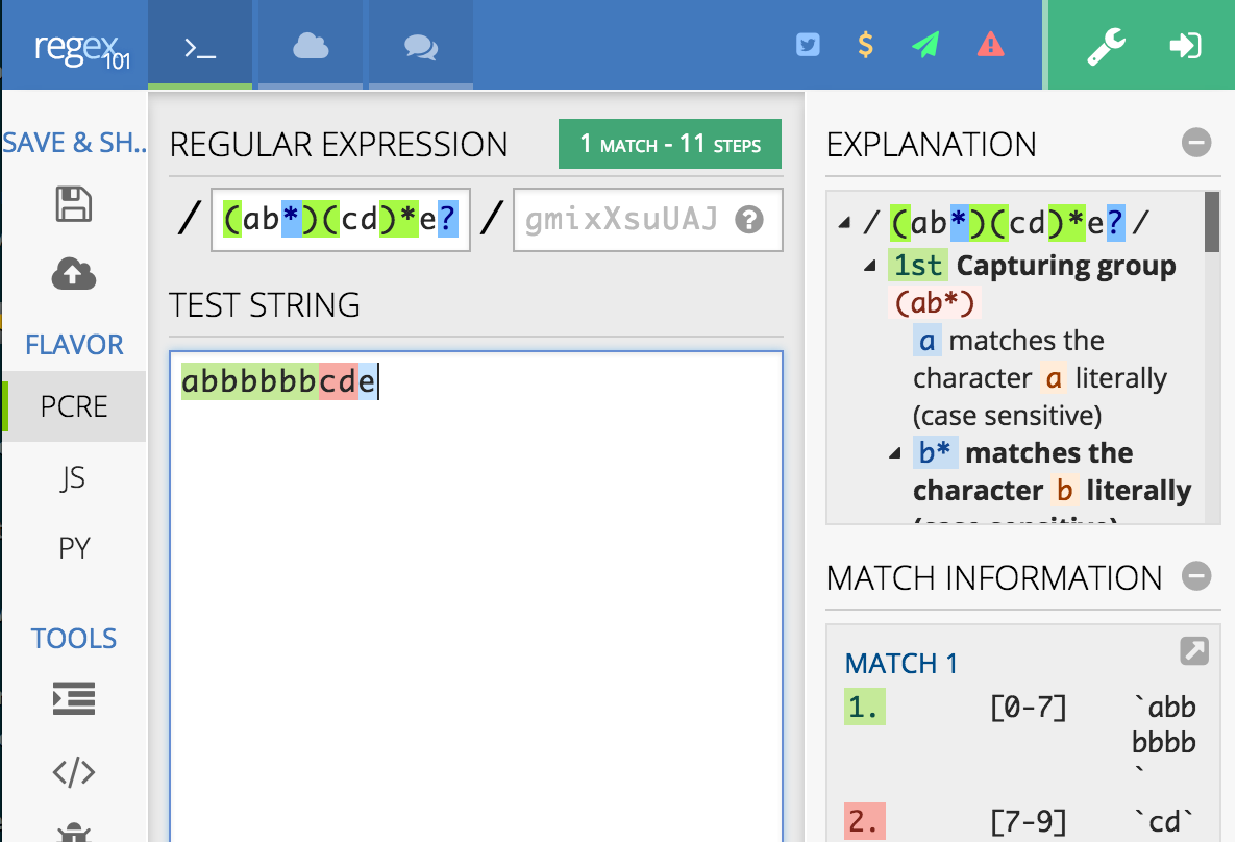
\includegraphics[scale=0.35]{nontex/regex101}
  \label{fig:regex101}
\end{figure}
\begin{center}
50\% say they use testing tools like www.regex101.com
\end{center}
\end{frame}
\note[itemize]{
    \item pt 1
    \item pt 2
}

%------------------------------------------------


% \begin{frame}[fragile]
% \frametitle{Parsing HTML}
% \begin{center}
% Only 28\% (5) admit to using regex to parse HTML.
% \end{center}
% \begin{center}
% \cverb!<li><a href="([^"]*)">([^"]*)</a></li>!
% \end{center}
% \begin{table}
% \begin{tabular}{l l l}
% \toprule
% & \textbf{NParticipants} & \textbf{\%} \\
% \midrule
% "use only custom parser" & 4 & 22\% \\
% "use only regex" & 2 & 11\% \\
% "it depends" & 12 & 67\% \\
% \bottomrule
% \end{tabular}
% \caption{Would you rather use regex or a custom parser?  }
% \begin{block}{If it depends, why?}
% \emph{parsers are more powerful than regex, if the problem can be solved with regex I prefer regex...}
% \\* \emph{If this is a one off application than a regex will work fine.}
% \end{block}
% \end{table}

% \end{frame}
% \note[itemize]{
%     \item Of those who said it depends, there was much agreement that parsers are more powerful, better at handling complexity, and provide more readable code. Regexes were mentioned positively for handling less structured inputs, form validation and ‘one-off’ programs
% }

% %------------------------------------------------

%\begin{frame}
%\frametitle{Usage Frequency - By Technical Environment}
%\begin{center}
%Heaviest regex use is in command line tools and text editors.
%\end{center}
%\begin{adjustbox}{width=\textwidth}
\begin{tabular}{l | r @{  } r @{  } r @{  } r @{  } r @{  } r }
\toprule
\textbf{Language/Environment} & \textbf{0} & \textbf{1-5} & \textbf{6-10} & \textbf{11-20} & \textbf{21-50} & \textbf{51+} \\  \midrule
General  (e.g., Java)  & 1 & 6 & 5 & 3& 1& 2 \\ \midrule
Scripting  (e.g., Perl) &5 &4 &3 &3 &2  &1 \\ \midrule
Query  (e.g., SQL) & 15&2 &0 &0 &1  & 0\\ \midrule
Command line (e.g., grep)   &2 &5 &3 &2 &0  &\textcolor{red}{6} \\ \midrule
Text editor (e.g., IntelliJ)   & 2& 5& 0& 5& 1& \textcolor{red}{5}\\
\bottomrule
\end{tabular}
\end{adjustbox}

%\end{frame}
%\note[itemize]{
%    \item Only 27\% (5) of participants wrote regular expressions that persist (general purpose, scripting, etc.) more frequently than in a text editor or command line tool (where they will not persist).
%}
%
%%------------------------------------------------
%
%
%\begin{frame}
%\frametitle{Ephemeral vs Persistent Users}
%\begin{adjustbox}{width=\textwidth}
\begin{tabular}{lccc}
\toprule
\textbf{Task} & \textbf{Persistence Freq.} & \textbf{Ephemeral Freq.} & \textbf{Difference} \\  \midrule
Counting  substrings that match a pattern & 3 & 1.7 & 1.2\\  \midrule
Parsing user input & 3.6 & 2.7 & 0.9\\ \midrule
Capturing parts of strings & 3.8 & 3.1 & 0.7\\ \midrule
Parsing generated text & 2.4 & 1.9 & 0.5\\  \midrule
Locating content within a file or files & 3.6 & 3.2 & 0.4\\ \midrule
Filtering collections (lists, tables, etc.) & 2.2 & 1.9 & 0.3\\ \midrule
Counting lines that match a pattern & 1.8 & 2.1 & -0.3\\
\bottomrule
\end{tabular}
\end{adjustbox}

%\begin{table}
\caption{Survey results for regex usage frequencies, comparing persistent and ephemeral users \label{table:persistingFeatureGroups}}
\begin{center}
\begin{small}
\begin{tabular}{llccc}
\toprule
\textbf{Group} & \textbf{Code} &  \textbf{Ephemeral Users} & \textbf{Persistent Users} & \textbf{Difference}\\  \midrule \bigstrut
\multirow{2}{*}{(neg) look-ahead/behind} &  (LKA, NLKA,  & \multirow{2}{*}{2.2} & \multirow{2}{*}{3.2} & \multirow{2}{*}{1.0} \\
& LKB, NLKB) & &\\
\midrule \bigstrut
lazy repetition & (LZY) &  2.8 & 3 & 0.2\\
\midrule \bigstrut
endpoint anchors & (STR, END) & 4.4 & 4.4 & 0\\ \midrule \bigstrut
capture groups & (CG) & 4.2 & 4.2 & 0\\ \midrule \bigstrut
word boundaries & (WNW) & 3.5 & 3.4 & -0.1\\
\bottomrule
\end{tabular}
\end{small}
\end{center}
\vspace{-12pt}
\end{table}

%\end{frame}
%\note[itemize]{
%    \item The five persistent users have an average of 12.4 years of experience. This contrasts with an average of 7.7 years of experience for ephemeral users. Considering usage frequency, 60\% (3) of the five persistent users indicate using regex weekly, vs 46\% (6) of the 13 ephemeral users.
%    \item In the case of the most rarely-used feature asked about, the OPT feature, three of the four participants who have ever used the OPT feature are persistent users
%}
%
%------------------------------------------------

\begin{frame}
\frametitle{Pain points}
\begin{block}{hard to compose (11 = 61\%)}
\emph{...very difficult to write them since I`ve never read up on them.}
%\\*\emph{...trickiness to getting the expression right}
\end{block}
\onslide<2->
\begin{block}{hard to read (7 = 39\%)}
%\emph{long ones can be hard to read}
%\\*\emph{Readability. Edge cases.}
\emph{It is terrible to read (especially later after initial development) }
\end{block}
\onslide<3->
\begin{block}{inconsistency across implementations (3 = 17\%)}
%\emph{Differences in implementation across languages}
\emph{Some regexes work differently (or don`t work) in some languages.}
\end{block}
\end{frame}
\note[itemize]{
    \item pt 1
    \item pt 2
}

%------------------------------------------------


\begin{frame}
\frametitle{Notable observations: Context}

\begin{block}{}
\begin{itemize}
	\item {\em Everyone} (sort of) {\em writes regexes} regularly 
	\item Developers find regexes {\em hard to read and write}
	\item Most often written in text editors and IDEs
	\item Testing regexes is {less} common than testing other code
\end{itemize}
\end{block}

\onslide<2->
but....

\onslide<3->
\begin{block}{}
%How do developers \emph{really} use regexes? 
\begin{itemize}
\item Are regexes everywhere?
\item Which features are everywhere?
\end{itemize}
\end{block}



\end{frame}









